% Aquí definí algunos comandos personalizados.
% Los más importantes son: \latt que escribe L(B) y
% \lattprime -> L(B').
% Otros son \ZZ, \RR, \QQ etc. que escriben los enteros, reales
% etc.
\documentclass{beamer}

\usepackage{subcaption, float}
\usepackage{graphicx} % Required for inserting images
\usepackage{svg}
\usepackage[spanish]{babel}

%%%%%%%%%% Font %%%%%%%%%%%
\usepackage[T1]{fontenc}
\usepackage{amssymb, amsfonts}
\usepackage{amsbsy}
%%%%%%%%%%%%%%%%%%%%%%%%%%%


%%%%%%%%%% Math %%%%%%%%%%%
% Useful tools like equation environments, alignment, etc.
\usepackage{amsthm, amsmath}

% Para cambiar a los símbolos "tradicionales" de
% de los naturales reales etc. se tiene que cambiar
% \mathbf por \mathbb. Me gusta más dejarlos en negrita
% porque encuentro que es más legible en presentaciones,
% pero si quieren lo cambian.
\newcommand{\ZZ}{\mathbf{Z}}
\newcommand{\QQ}{\mathbf{Q}}
\newcommand{\RR}{\mathbf{R}}
\newcommand{\MM}{\mathbf{M}}
\newcommand{\NN}{\mathbf{N}}
\newcommand{\latt}{\mathcal{L}(\mathbf{B})}       % Para escribir menos
\newcommand{\lattprime}{\mathcal{L}(\mathbf{B'})} % Para escribir menos

%%%%%%%%%%%%%%%%%%%%%%%%%%%%


%%%% Beamer specific %%%%%%
\title{Introducción a Reticulados}
% Pongan sus apellidos maternos en ...
\author{Leandro Aballay Henríquez, Diego Cuevas Alarcón, Matías Olivares Morales, Álvaro Quezada Inostroza, Guillermo Pereira Bula}
\institute{Departamento de Matemática y Ciencia de la Computación\\}
\date{17 de julio de 2025}

\AtBeginSection[]
{
  \begin{frame}
    \frametitle{Contenidos}
    \tableofcontents[currentsection]
  \end{frame}
}

\uselanguage{Spanish}
\languagepath{Spanish}
\newcommand{\adv}[1]{ {\color{blue} #1} }


\usetheme{default}
\usecolortheme{default}
%%%%%%%%%%%%%%%%%%%%%%%%%%%


\begin{document}
\frame{\titlepage}

\begin{frame}
\frametitle{Contenidos}
\tableofcontents
\end{frame}

\section{Marco teórico}
\subsection{Definiciones básicas}
% Por ahora estoy poniendo las cosas nomas. De ahí les podemos poner titulo
% a los frames o q se yo, refinar la presentacion etc.
\begin{frame}{Reticulado}
\only<1>{
\begin{definition}
Sea $\RR^m$ el espacio euclidiano $m$-dimensional. Un reticulado en $\RR^m$ es el conjunto
\[
\mathcal L(\mathbf{b}_1, \dots, \mathbf{b}_n) = \left\{\sum_{i = 1}^n x_i \mathbf{b}_i : x_i  \in \ZZ\right\}
\]
De combinaciones lineales enteras de $n$ vectores linealmente independientes $\mathbf{b}_1, ..., \mathbf{b}_n$ en $\RR^m$ con $m \geq n$.
\end{definition}
Llamamos a los enteros $m$ y $n$ como {\it dimensión} y {\it rango} respectivamente. Si $m = n$, es decir, si el número de vectores base es igual a la dimensión del espacio, entonces diremos que $\latt$ es de rango completo, o dimensión completa.
}

\only<2>{Los vectores $\mathbf{b}_1, ..., \mathbf{b}_n$ son la {\it} base del reticulado. Podemos representarlos como una matriz $\RR^{m\times n}$ donde los vectores base ``se ven'' como columnas

\[
\mathbf{B} = \begin{bmatrix}
    \mathbf{b}_1 & \dots & \mathbf{b}_n
\end{bmatrix}
\]

De esta forma compactamos la primera definición como $\mathcal{L}(\mathbf B) = \left\{\mathbf{Bx} : \mathbf x \in \ZZ^n\right\}$. 

Un reticulado tiene muchas bases distintas. Dos bases $\mathbf B$ y $\mathbf B'$ que generan el mismo reticulado se dicen {\it equivalentes}.
}
\only<3>{
\begin{figure}
    
    \centering
    
    \begin{subfigure}{0.4\textwidth}
        \includesvg[width=\linewidth]{figures/lattice_fig.svg}
        \caption{$\mathbf B = [\mathbf b_1\quad \mathbf b_2]$}
        \label{fig:simple_lattice}
    \end{subfigure}
    \hfill
    \begin{subfigure}{0.4\textwidth}
        \includesvg[width=\linewidth]{figures/lattice_bprime.svg}
        \caption{$\mathbf B' = [\mathbf b'_1\quad \mathbf b'_2]$}
        \label{fig:same_basis}
    \end{subfigure}
    \caption{Dos bases equivalentes.}
\end{figure}
}
\end{frame}

\begin{frame}{Amplitud}
La {\it amplitud} (o {\it span}) de la base de un reticulado se define como el conjunto de todas las combinaciones lineales {\it reales} de los vectores base:
\[
\text{span}(\mathbf B) = \left\{\mathbf{Bx} : \mathbf x \in \RR^n \right\}
\]

$\mathbf B$ es una base para $\text{span}(\mathbf{B})$ visto como un espacio vectorial. En particular, esto implica que $\text{rank}(\latt) = \text{dim}(\text{span}(\mathbf B))$. Asimismo, $\text{span}(\mathbf B) = \RR^m$ si su dimensión es $m$. De lo anterior podemos concluir que $\latt$ es de rango completo si y solo si $\text{span}(\mathbf B) = \RR^m$.

\begin{remark}
Cualquier conjunto de $n$ vectores L.I. $\mathbf B'$ del reticulado $\latt$ es una base para $\text{span}(\mathbf B)$, pero $\mathbf B'$ no es necesariamente equivalente a $\mathbf B$.
\end{remark}
\end{frame}

\begin{frame}{Otra representación de reticulados}
También podemos caracterizar un reticulado sin hacer uso de una base $\mathbf B$, mediante teoría de grupos. Consideremos un reticulado como un $\Lambda \subseteq \RR^m$ no vacío, y cerrado bajo la resta.

\begin{proposition}
    Un reticulado $\Lambda$ es un subgrupo aditivo discreto de $\RR^m$.
\end{proposition}
\begin{proof}
    Por definición $\Lambda \subseteq \RR^m$. Luego, por el criterio de subgrupo, basta con mostrar que $\Lambda$ es cerrado bajo la inversión y la suma.

    Sea $\mathbf x, \mathbf y \in \Lambda$, entonces $\mathbf 0 \in \Lambda$ porque $\mathbf x - \mathbf x \in \Lambda$. Sigue inmediatamente que $\mathbf{0 - x} = \mathbf {-x} \in \Lambda$. Por último, $\mathbf{x+y} = \mathbf x - (-\mathbf y) \in \Lambda$.
\end{proof}

Aquí, {\it discreto} significa que existe una constante real positiva $\lambda$ tal que la distancia entre dos vectores cualquiera del reticulado es, al menos, $\lambda$.
\end{frame}

\begin{frame}{Equivalencia de bases}
\only<1>{
La equivalencia de bases de reticulados se puede interpretar de forma geométrica. Defina el paralelepípedo semiabierto de $\mathbf B$ como el conjunto

\[
\mathcal P(\mathbf B) = \left\{ \mathbf B\mathbf x : 0 \leq x_i < 1\right\}.
\]

Sea $\mathbf B'$ una matriz de vectores L.I. de $\latt$, entonces $\mathbf B'$ es una base para $\latt$ si y solo si $\mathcal P(\mathbf B')$ no contiene ningún vector de $\latt$ además del origen.
}
\only<2>{
\begin{figure}
    \centering
    \includesvg[width=0.55\linewidth]{figures/lattice_parallelepiped.svg}
    \caption{$\mathcal P(\mathbf B')$ contiene $\mathbf b_1$ y $2 \mathbf b_1$, por lo tanto la base propuesta no genera el mismo reticulado.}
    \label{fig:parallelepiped}
\end{figure}
}
\end{frame}

% La corta demostración
\begin{frame}
\only<1>{
\begin{theorem}
Sean $\mathbf B$ y $\mathbf B'$ dos bases $\RR^{m \times n}$. $\mathbf B$ y $\mathbf B'$ son equivalentes si y solo si existe una matriz unimodular $\mathbf U \in \ZZ^{n \times n}$ tal que $\mathbf B = \mathbf {B' U}$
\end{theorem}
}
\begin{proof}
 \only<1>{$(\impliedby)$ Tenemos que $\mathbf B = \mathbf{B'U}$ y $\det(\mathbf U) = \pm 1 \neq 0$, entonces $\mathbf U$ es invertible por alguna matriz $\mathbf U'$ tal que $\mathbf{UU'} = \mathbf I$. En particular, de esto podemos concluir que $\mathbf{B'} = \mathbf{BU'}$. Sigue inmediatemente que $\latt \subseteq \lattprime$ y $\lattprime \subseteq \latt$. Por lo tanto $\latt = \lattprime$ y ambas bases son equivalentes.}

 \only<2>{$(\implies)$ Si $\mathbf B$ y $\mathbf B'$ son equivalentes entonces generan el mismo reticulado. Es decir, existen $\mathbf M$ y $\mathbf M' \in \ZZ^{n\times n}$  tal que $\mathbf B = \mathbf{B'M'}$ y $\mathbf B' = \mathbf{BM}$.
 \[
 \mathbf B = \mathbf{BMM'} \implies \mathbf{B}(\mathbf{I - MM'}) = \mathbf 0
 \]
 Sabemos que $\mathbf B$ es linealmente independiente. Por lo tanto $(\mathbf{I- MM'}) = \mathbf 0$. Luego 
\[ 
 \det(\mathbf{MM'}) = \det(\mathbf M) \cdot \det(\mathbf M') = \det(\mathbf{I}) = 1
 \]

Como $\mathbf M$ y $\mathbf M'$ están compuestas de enteros, $\det(\mathbf M)$ y $\det(\mathbf{M'})$ deben ser enteros. Como la multiplicación de ambos determinantes debe ser uno, entonces solo pueden ser $1$ o $-1$. Por lo tanto $\mathbf M$ y $\mathbf M'$ son unimodulares
 }
 \alt<2>{\qedhere}{\phantom\qedhere}
\end{proof}
\end{frame}

\subsection{Determinantes}
\begin{frame}{Determinante}
\begin{definition}
El determinante de un reticulado $\Lambda = \latt$ es el volumen $n$-dimensional del paralelepípedo semiabierto $\mathcal P(\mathbf B)$.
\end{definition}

El determinante es invariante, es decir, no depende de la elección de base. Una forma de computar $\text{det}(\Lambda)$ es mediante la ortogonalización Gran-Schmidt. Sea $\mathbf B^* = [\mathbf b_1^*, \dots, \mathbf b_n^*]$ la matriz de vectores ortogonalizados de una base $\mathbf B$.

\[
\det(\Lambda) = \prod_{i = 1}^n ||\mathbf b_i^*||
\]

Si $\latt = \Lambda$ es de rango completo entonces $\det(\Lambda) = |\det(\mathbf B)|$.

\end{frame}


\subsection{Mínimos sucesivos}
\begin{frame}{Mínimos sucesivos}
\only<1>{
    \begin{definition}
        $\mathcal{B}_m(\mathbf{0},r) = \left\{ \mathbf{x} \in \RR^{m}: \Vert \mathbf{x} \Vert < r \right\}$ es la \textbf{esfera abierta} $m$-dimensional de radio $r$ y centrada en $\mathbf{0}$.
    \end{definition}
    
    \begin{definition}
        Llamamos \textbf{mínimos sucesivos} a la sucesión de valores $\lambda_1, \dots, \lambda_n$ tal que se cumple
        $$ 
        \lambda_i(\Lambda) = \inf\{r: \dim(\text{span}(\Lambda \cap \mathcal{B}_m(\mathbf{0},r))) \geq i\}
        $$
    
        En otras palabras, el $i$-ésimo mínimo $\lambda_i$ corresponde al radio de la esfera abierta más pequeña, centrada en el origen, que contiene al menos $i$ vectores linealmente independientes.  
    \end{definition}
}

\only<2>{
\begin{figure}
    \centering
    \includesvg[width=0.55\linewidth]{figures/minima.svg}
    \caption{Segundo mínimo.}
    \label{fig:enter-label}
\end{figure}
}

\only<3>{
    Los mínimos sucesivos pueden definirse respecto a cualquier tipo de norma, siempre y cuando cumpla ciertas propiedades (definida positiva, ponderación por escalar y desigualdad triangular). Algunos ejemplos son:
    \vspace{10pt}
    \begin{itemize}
        \item norma $\ell_1$: \quad ${\Vert\mathbf{x}\Vert}_1 = \sum |x_i|$
        \vspace{7pt}
        \item norma $\ell_2$: \quad ${\Vert\mathbf{x}\Vert}_2 = \sqrt{\sum x^2_i} = \sqrt{\langle \mathbf{x},\mathbf{x} \rangle}$
        \vspace{7pt}
        \item norma $\ell_{\infty}$: \quad ${\Vert\mathbf{x}\Vert}_{\infty} = \displaystyle \lim_{p \to \infty} {\Vert\mathbf{x}\Vert}_p = \max_{i=1}^n |\mathbf{x}_i|$
    \end{itemize}
}

\only<4>{
\begin{remark}
    Ya que $\Lambda \subseteq \RR^m$, siempre existen vectores que cumplen la sucesión mínima, es decir, existen $\mathbf b_1, \dots, \mathbf b_n$ L.I. en $\Lambda$ tal que $||\mathbf b_i|| = \lambda_i$ para todo $i = 1,\dots,n$. Esto implica que el ínfimo de la definición de $\lambda_i(\Lambda)$ es un mínimo si se reemplaza $\mathcal B_m(\mathbf 0, r)$ por la esfera {\it cerrada} $\overline{\mathcal B}(\mathbf 0, r)$.
\end{remark}

Por otro lado, $\lambda_1(\Lambda)$ es el largo del vector distinto de cero más corto del reticulado, y es igual a la distancia más corta entre dos puntos distintos del reticulado. Formalmente:
\[
\lambda_1(\Lambda) = \min_{\mathbf x \neq \mathbf y \in \Lambda} || \mathbf x - \mathbf y|| = \min_{\mathbf x \in \Lambda \backslash \left\{\mathbf 0\right\}} ||\mathbf x||
\]
}
\end{frame}

\subsection{Teoremas de Minkowski}
\begin{frame}{Teoremas de Minkowski}
    \only<1>{
    \begin{theorem}{Teorema de Blichfeldt:} Para cualquier reticulado $\Lambda$ y para cualquier conjunto medible $S \subseteq span (\Lambda)$, si $S$ tiene un volumen $vol(S) > det(\Lambda)$ entonces existen dos puntos distintivos $z_1, z_2 \in S$ tal que $z_1 - z_2 \in \Lambda$.
    \end{theorem}
    \begin{theorem}{Primer Teorema de Minkowski:}
        Para cualquier reticulado $\Lambda$ de rango $n$ y dado cualquier conjunto convexo y simétrico al origen $S \subset span(\Lambda)$, si $vol(S)> 2^n det(\Lambda)$ entonces $S$ contiene un punto no-nulo $v$ del reticulado tal que $v \in S \cap \Lambda \backslash {0}$  
    \end{theorem}
    }
    \only<2>{
    \begin{remark}
        Para cualquier reticulado $\Lambda$ de rango $n$, el largo del vector más corto sin considerar el vector del punto origen es $\lambda_1 < \sqrt{n} \ det(\Lambda)^{1/n}$ 
    \end{remark}
    \begin{theorem}{Segundo Teorema de Minkowski:}
        Para cualquier reticulado $\latt$ con rango $n$, los mínimos sucesivos (en norma $\ell_2$) $\lambda_1, \dots, \lambda_n$ satisfacen
        \[
            (\prod_{i=1}^{n} \lambda_i)^{1/n} < \sqrt{n} \ det(\mathbf B)^{1/n}
        \]
    \end{theorem}
    }
\end{frame}

\section{Algunos problemas computacionales de reticulados}

\subsection{SVP: El problema del vector más corto}
\begin{frame}{El problema del vector más corto}

El teorema de Minkowski solo nos dice que un vector corto no nulo existe en el reticulado, pero no nos entrega un método eficiente para encontrar vectores con largos acotados por $\sqrt{n}\det(\mathbf{\latt})^{1/n}$.

\begin{definition}[\textit{Shortest Vector Problem}, SVP]
Dada una base $\mathbf{B}\in \ZZ^{m\times n}$, encontrar el vector no nulo del reticulado $\mathbf{Bx}$ (con $\mathbf{x}\in\ZZ^n\setminus\{\mathbf{0}\}$) tal que $\|\mathbf{Bx}\| \leq \|\mathbf{By}\|$ para cualquier otro vector $\mathbf{y}\in\ZZ^n\setminus\{\mathbf{0}\}$. 
\end{definition}

\begin{definition}[SVP Aproximado]
Dada una base $\mathbf{B}\in \ZZ^{m\times n}$, encontrar el vector no-nulo del reticulado $\mathbf{Bx}$ (con $\mathbf{x}\in\ZZ^n\setminus\{\mathbf{0}\}$) tal que $\|\mathbf{Bx}\| \leq \gamma \cdot \|\mathbf{By}\|$ para cualquier otro vector $\mathbf{y}\in\ZZ^n\setminus\{\mathbf{0}\}$.
\end{definition}

En esta versión de optimización, solo es necesario encontrar $\|\mathbf{Bx}\|$; es decir, un valor $d$ tal que $\lambda_1(\mathbf{B}) \leq d < \gamma\lambda_1(\mathbf{B})$.
\end{frame}

\begin{frame}{SVP en dos dimensiones}
    \begin{definition}
        Sea $[\textbf{a},\textbf{b}]$ una base de un reticulado. La base es reducida si
        \[
            ||\textbf{a}||,||\textbf{b}|| \leq ||\textbf{a}+\textbf{b}||,||\textbf{a}-\textbf{b}|| \text{.}
        \]
        \begin{figure}
            \centering
            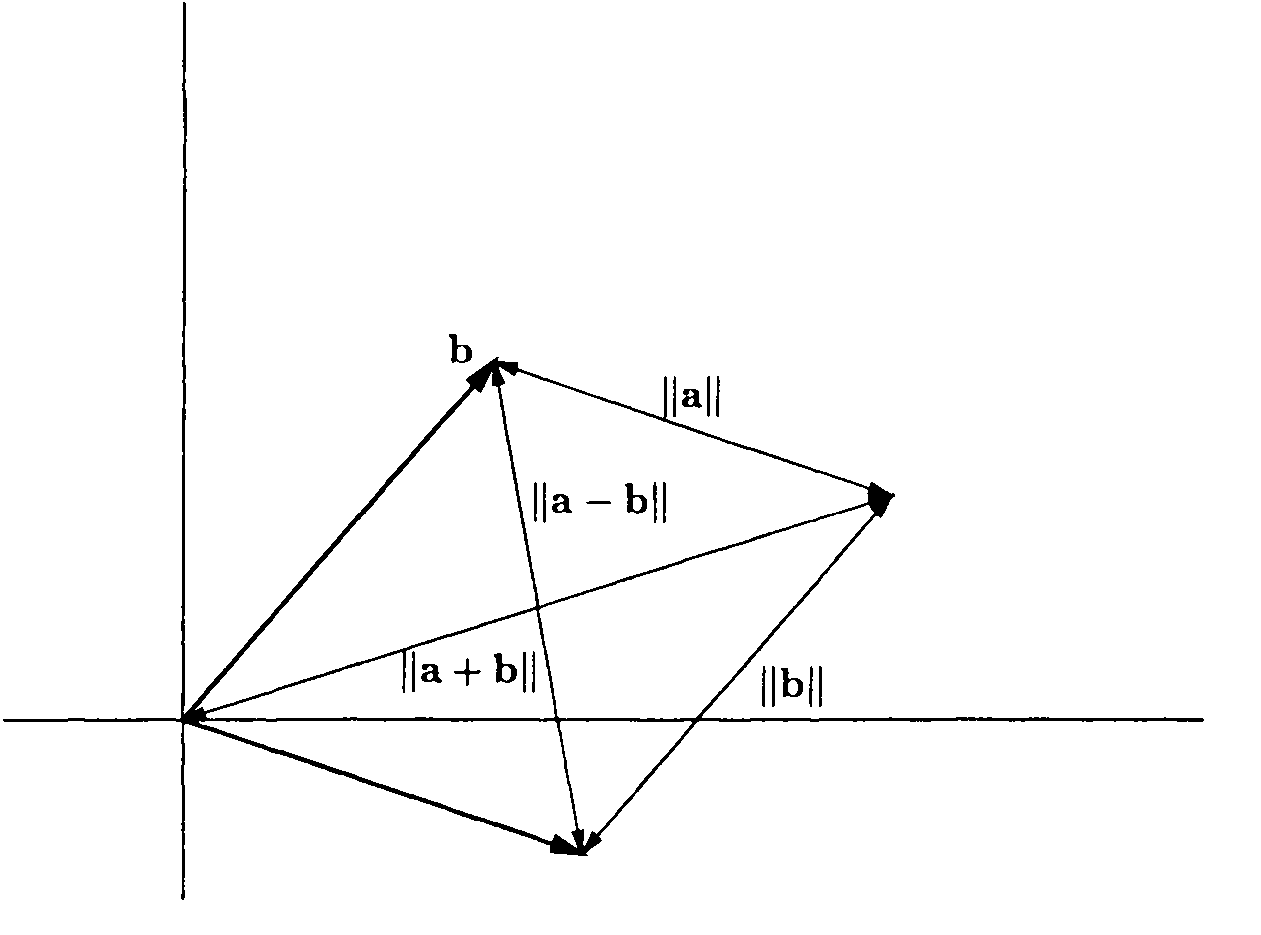
\includegraphics[width=0.5\linewidth]{figures/baseReducida.png}
            \caption{Base reducida en dos dimensiones}
        \end{figure}
    \end{definition}
\end{frame}

\begin{frame}
    \begin{lemma}
        Considere tres vectores en una linea, $\textbf{x}, \textbf{x}+\textbf{y}, \textbf{x}+\textbf{$\alpha$} \textbf{y}$, donde $\alpha \in (1, \infty)$. Para cualquier norma $||\cdot||$, si $||\textbf{x}|| \leq ||\textbf{x}+\textbf{y}||$ entonces $||\textbf{x}+\textbf{y}|| \leq ||\textbf{a}+\alpha \textbf{y}||$. Además, si $||\textbf{x}||<||\textbf{x}+\textbf{y}||$ entonces $||\textbf{x}+\textbf{y}||<||\textbf{x}+\alpha \textbf{y}||$.
    \end{lemma}
    \begin{figure}
        \centering
        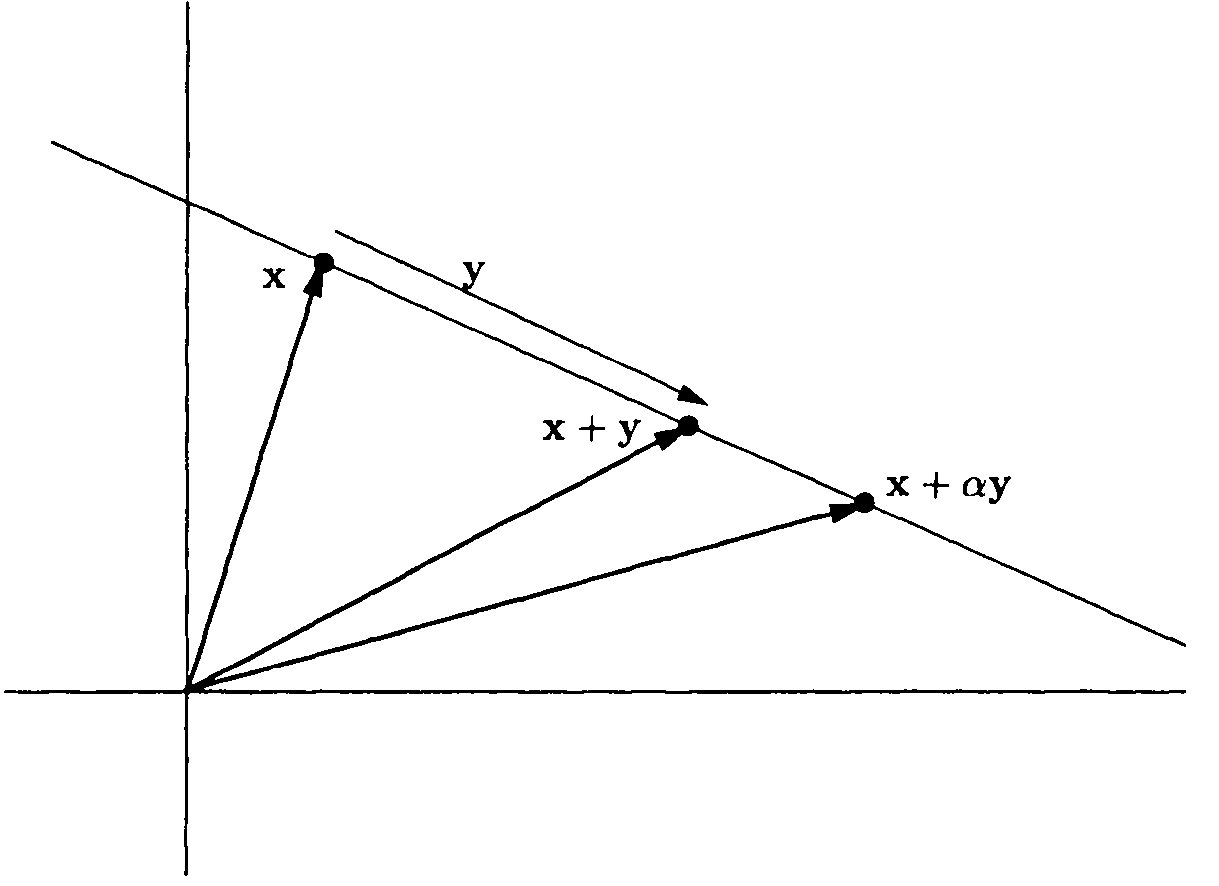
\includegraphics[width=0.45\linewidth]{figures/lattice_pointsLine.png}
        \caption{Tres puntos en una línea}
    \end{figure}
\end{frame}

\begin{frame}{Algoritmo generalizado de Gauss}
Algoritmo utilizado para reducir la base de un reticulado. 
    \begin{figure}
        \centering
        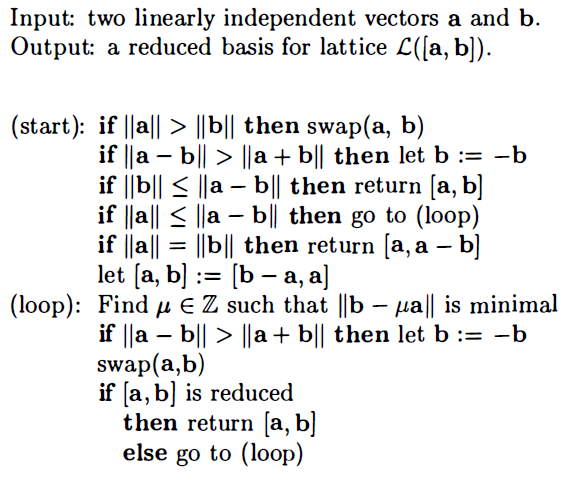
\includegraphics[width=0.65\linewidth]{figures/lattice_gaussAlg.png}
        \caption{Generalización del algoritmo de Gauss}
    \end{figure}
\end{frame}

\begin{frame}{Algoritmo generalizado de Gauss}
Del algoritmo presentado para la reducción de base en dos dimensiones podemos decir:
\begin{itemize}
    \item El algoritmo es de complejidad $O(n)$.
    \item El algoritmo es eficiente y exacto para encontrar el vector más corto.
    \item Es genérico respecto a la norma siempre y cuando esta pueda ser evaluada en tiempo polinomial.
    \item Se basa en propiedades geométricas del reticulado. 
\end{itemize}
\end{frame}

\subsection{CVP: El problema del vector más cercano}

\begin{frame}{El problema del vector más cercano}
\begin{definition}[\textit{Closest Vector Problem}, CVP]
Dada una base $\mathbf{B}\in \ZZ^{m\times n}$ y un vector objetivo $\mathbf{t} \in \ZZ^m$, encontrar el vector no nulo del reticulado $\mathbf{Bv}$ más cercano a $\mathbf{t}$; es decir, encontrar un vector $\mathbf{v}\in \ZZ^n$ de modo que $\|\mathbf{Bv}-\mathbf{t}\| \leq \|\mathbf{Bw}-\mathbf{t}\|$ para cualquier otro $\mathbf{w} \in \ZZ^n$.
\end{definition}
\begin{figure}
    \centering
    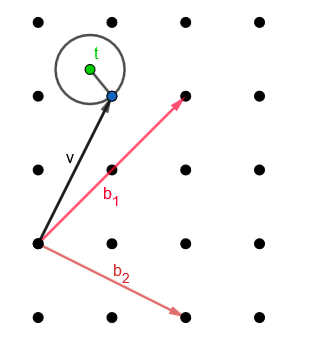
\includegraphics[width=0.35\linewidth]{figures/The-closest-vector-problem.png}
    \caption{\textit{Closest Vector Problem}}
    \label{fig:cvp-figure}
\end{figure}

\end{frame}

\begin{frame}{El problema del vector más cercano}
El problema de encontrar el vector más cercano se puede abordar mediante las siguientes tareas computacionales:

\begin{itemize}
    \item \textit{Problema de Búsqueda}: Dado un reticulado entero $\latt$ y un vector objetivo $\mathbf{t}$, encontrar un vector del reticulado $\mathbf{Bx}$ tal que $\|\mathbf{Bx} - \mathbf{t}\|$ sea mínima.
    \item \textit{Problema de Optimización}: Dado un reticulado entero $\latt$ y un vector objetivo $\mathbf{t}$, computar $\text{dist}(\mathbf{t}, \latt)$.
    \item \textit{Problema de Decisión}: Dado un reticulado entero $\latt$, un vector objetivo $\mathbf{t}$ y un racional $r$, determinar si $\text{dist}(\mathbf{t}, \latt) \leq r$ o $\text{dist}(\mathbf{t}, \latt) > r$.
\end{itemize}
\end{frame}

\begin{frame}{El problema del vector más cercano}
\begin{remark}
Dada una máquina que resuelve el problema de decisión (NP-completo), se puede resolver el problema de búsqueda en tiempo polinomial.
\end{remark}

Para esto, suponemos que tenemos un algoritmo $\mathcal{A}$ que, para una entrada $(\mathbf{B},\mathbf{t},r)$, decide si $\text{dist}(\mathbf{t}, \latt) \leq r$ o $\text{dist}(\mathbf{t}, \latt) > r$, y lo utilizamos para encontrar de manera eficiente un punto $\mathbf{Bx}$ del reticulado más cercano a $\mathbf{t}$, para una base $\mathbf{B}$ y un vector objetivo $\mathbf{t}$ de entrada.

De manera similar, dado un algoritmo de optimización que computa $\text{dist}(\mathbf{t},\latt)$, se puede resolver el problema de decisión $(\mathbf{B}, \mathbf{t}, r)$ comparando $\text{dist}(\mathbf{t},\latt)$ con $r$.
\end{frame}

\begin{frame}{El problema del vector más cercano}
\begin{definition}[CVP Aproximado]
Dada una base $\mathbf{B}\in \ZZ^{m\times n}$ y un vector objetivo $\mathbf{t} \in \ZZ^m$, encontrar el vector no nulo del reticulado $\mathbf{Bx}$ (con $\mathbf{x}\in \ZZ^n$) de modo que $\|\mathbf{Bx}-\mathbf{t}\| \leq \gamma \cdot \|\mathbf{By}-\mathbf{t}\|$ para cualquier otro $\mathbf{y} \in \ZZ^n$.
\end{definition}

En esta versión de aproximación, solo es necesario encontrar $\|\mathbf{Bx}-\mathbf{t}\|$; es decir, un valor $d$ tal que $\text{dist}(\mathbf{t},\latt) \leq d < \gamma \cdot \text{dist}(\mathbf{t},\latt)$.
A la fecha, los algoritmos de aproximación más eficientes (los de aleatoriedad posiblemente) para CVP utilizan factores de aproximación polinomiales $\gamma(n) = n^c$ (para algún $c$ independiente del rango $n$) en el peor caso.

\end{frame}

\subsection{LLL}
\begin{frame}{Algoritmo LLL}
    \begin{itemize}
        \item Es un algoritmo de aproximación para el problema del vector más corto, que se ejecuta en tiempo polinomial
    \end{itemize}
\end{frame}

\begin{frame}{Algoritmo LLL}
    \begin{algorithmic}
    \State \textbf{Entrada:} Reticulado con base \textbf{b$_1$, $\dots$, b$_n$} $\in \mathbb{Z}^n$
    \State \textbf{Salida:} $\delta$-LLL base reducida de $\mathcal{L}$
    \State \textbf{Comienzo:} computar Gram-Schmidt \textbf{b}$_1^*$, $\dots$, \textbf{b}$_n^*$
    \State \textbf{Paso de Reducción:}
    \For{$i=2$ to $n$} 
        \For{$j = i − 1$ to $1$}
            \State $b_i \gets b_i - c_{ij}b_ji$, donde $c_{ij} = \frac{\langle b_i, b^*_j \rangle}{\langle b^*_j,b^*_j \rangle}$ 
        \EndFor
    \EndFor
    \State \textbf{Paso Swap:} \Comment{Verificar condición de Lovász}
    \If{$\exists i$ tal que $\delta ||b^*_i||^2 > ||\mu_{i+1, i}b^*_i + b^*_{i+1}||^2$}
        \State $b_i\leftrightarrow b_{i+1}$
    \EndIf
    \end{algorithmic}
\end{frame}

\begin{frame}
    \begin{center}
        {\huge \bf Preguntas}
    \end{center}
\end{frame}
\end{document}
